% LaTeX Article Template - customizing header and footer
\documentclass{article}

\newtheorem{thm}{Theorem}

% Set left margin - The default is 1 inch, so the following 
% command sets a 1.25-inch left margin.
\setlength{\oddsidemargin}{0.25in}

% Set width of the text - What is left will be the right margin.
% In this case, right margin is 8.5in - 1.25in - 6in = 1.25in.
\setlength{\textwidth}{6in}

% Set top margin - The default is 1 inch, so the following 
% command sets a 0.75-inch top margin.
\setlength{\topmargin}{-0.25in}

% Set height of the header
\setlength{\headheight}{0.3in}

% Set vertical distance between the header and the text
\setlength{\headsep}{0.2in}

% Set height of the text
\setlength{\textheight}{9in}

% Set vertical distance between the text and the
% bottom of footer
\setlength{\footskip}{0.1in}

% Set the beginning of a LaTeX document
\usepackage{multirow}
\usepackage{fullpage}
\usepackage{graphicx}
\usepackage{amsthm}
\usepackage{url}
\usepackage{amssymb}
\usepackage{amssymb}
\usepackage{algpseudocode}
\graphicspath{%
    {converted_graphics/}% inserted by PCTeX
    {/}% inserted by PCTeX
}
%%%%%%%%%%%%%%%%%%%%%%%%%%%%%




\begin{document}\title{Homework $1$\\ Computer Science \\ B551 Spring 2018\\ Hasan Kurban}         % Enter your title between curly braces
\author{Jinju Jiang(Hellen)}        % Enter your name between curly braces
\date{\today}          % Enter your date or \today between curly braces
\maketitle


% Redefine "plain" pagestyle
\makeatother     % `@' is restored as a "non-letter" character




% Set to use the "plain" pagestyle
\pagestyle{plain}
\section*{Introduction}
The aim of this homework is to get you acquianted with problem solving and the steps  (Real World $\rightarrow$ Concept $\rightarrow$ Logic  $\rightarrow$ Implementation).  You will turn-in three files\begin{itemize} \item A *pdf with the written answers called \texttt{hw1.pdf} \item A Python script called \texttt{p1.py} for the drone scanning the floor plan \item  A Python script called  \texttt{p2.py} for rock-paper-scissors \end{itemize}  I am providing this \LaTeX{} document for you to freely use as well. Please enjoy this homework and ask yourself what interests you and then how can you add that interest to it!  Finally,  questions 3  and 4  are worth 50 points whereas questions 1 and 2 are 20  worth points.
\newpage
\section*{Homework Questions}
\begin{enumerate}
\item Problem 3.2 in the text.\\
\underline{Answer to question(a)}\\
we can formulate the problem as the following:\\
\textbf{States:} Let's use coordinate system to define the maze as the following: 2l is maze length, and 2w is maze width, initially the robot is in (0,0)position and is facing north. since robot can move any distance(continuous) and face 4 directions, so robot can be in any position except wall position.\\
\begin{figure}[h]
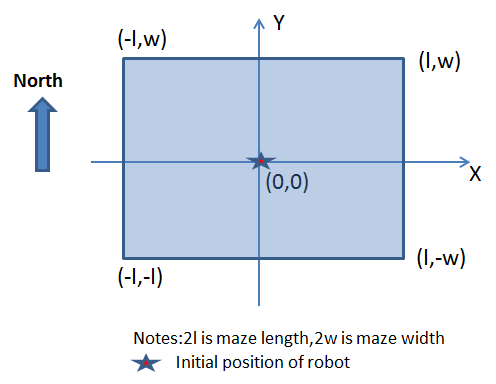
\includegraphics[width=0.4\columnwidth]{mazep1}\centering % Example image
\caption{Illustrate the robot maze in problem 1}
\end{figure}
\textbf{Initial State:} in position (0,0),facing North.\\
\textbf{Actions:} In this robot case, each state has 6 actions:face north, east, south, or west, and move or stop.\\
\textbf{Transition model or Successor function:} move any distance, change facing direction(north, east, south, or west).\\
\textbf{Goal test:} position is out of the maze, let's suppose position is (x,y), if $|x|>l$ or $|y|>w$, then it is goal status(outside of the maze).\\
\textbf{Cost function:} what we concern is that how long the robot will take to move to the outside of the maze, which is directly related with the distance it moved. So the cost function is the distance it moved.\\
\underline{Answer to question(b)}\\
\textbf{Initial State:} in position (0,0),facing North.\\
\textbf{Transition model or Successor function:} move to the next intersection if there is, or move to the end of corridor. Turn the directions((north, east, south, or west) at the intersections.\\
\textbf{States}:Since the robot will only change direction in intersection,otherwise it will keep moving until it encounter the end.So robot will stop at the end of corridor. let's support there are n ends of corridors, and there are m intersections,for each intersection, it can turn to 4 directions(north, east, south, or west), then state is n+4m.\\
\textbf{Goal test:}since the robot will go to the end of corridors or intersections, so we just need to check whether it is the exist node.\\
\textbf{Cost function:} total distance it moved.\\
\underline{Answer to question(c)}\\
\textbf{Initial State:} in position (0,0),facing North.\\
\textbf{Transition model or Successor function:} move to the next intersection and turn the directions((north, east, south, or west), or move to the end of corridor and turn directions.\\
\textbf{States}:n+4m(n is the ends nodes and m is number of intersections).\\
\textbf{Goal test:}check whether it is the exist node.\\
\textbf{Cost function:} total distance it moved.\\
No need to keep track of robot's orientation since it is not related with predicting the outcomes and it is not related to judge the goal state.\\
\underline{Answer to question(d)}\\
1.The first one is that there is enough power/batter to support robot to be in operation.\\
2.The second one is the ground is flat and smooth enough for robot to move(no obstacles to block robot moving).\\
3.The third one is that the robot can operate correctly, for example it can only face 4 directions, it can move in the same direction until it change the direction(only 4 directions).\\
\item Define {\it Artificial Intelligence} as rational behavior.  What is a problem that AI is {\it not} suited for?
\underline{Answer to question 2}\\
Given AI as rational behavior, then it is not suitable for "thinking" problems like psychological problems, congnitive problems, and emotional problems.\\
\item Assume you're programming an office security drone who's mission is to move through a floor, checking for any movement.  You've been given the floor plan shown below.  There are two entrances to the floor: \textsf{L, C}.  
\begin{center}
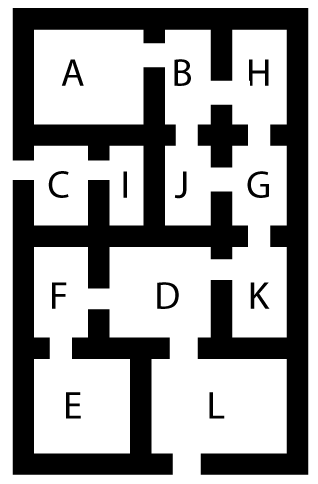
\includegraphics[scale=0.30]{maze55}
\end{center}
\begin{enumerate}
\item Using a graph $ G = (V,E)$, model this plan so that the drone can navigate the floor.  ({\it hint}) You'll need to have an additional vertex that represents the outside--call this vertex \textsf{U}.  $G$ is  an {\it undirected} graph (edges have no direction).  And edge is now either $\{u,v\}$ or $\{(u,v), (v,u)\}$.  This impacts the implementation.    For an adjancency list, you'll have to decide whether to have one edge or both. \\
\underline{Answer to question 3(a):}\\
$G=(V,E)$\\
$V=\{A,B,V,D,E,F,G,H,I,J,K,L,U\}$\\
$E={(A,B),(B,H),(B,J),(H,G),(G,J),(G,K),(U,C),(C,I),(F,D),(F,E),(D,L),(D,K),(L,U)}$\\
The graph is as the following:\\
\begin{figure}[h]
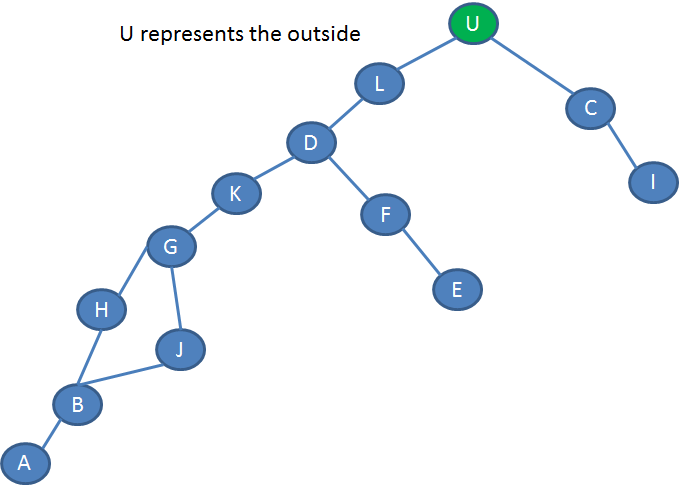
\includegraphics[width=0.5\columnwidth]{graphp3}\centering 
\caption{Illustrate the floor plan with graph}
\end{figure}
\item Using an adjacency list, model this floor plan.\\
\underline{Answer to question 3(b):}\\
For each vertex i i ii, store an array of the vertices adjacent to it.One adjacency list per vertex, U is additional vertex which represents the outside. So there 13 adjacency list including U by total. Here it is adjacency-list representation of the floor map.\\
\begin{figure}[h]
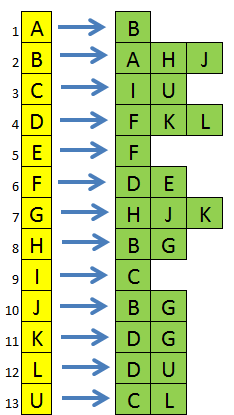
\includegraphics[width=0.3\columnwidth]{adjacentlistp3b}\centering 
\caption{Adjacency-list representation of the floor map}
\end{figure}
\item Trace a DFS on $G$ starting at \textsf{U}.\\
\underline{Answer to question 3(c):}\\
Here it is the stack table illustrating tracing a DFS on G starting at U:\\
\begin{figure}[h]
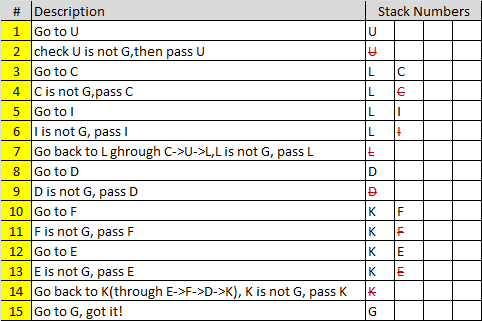
\includegraphics[width=0.6\columnwidth]{tracestackp3_1}\centering 
\caption{Illustrating tracing a DFS on G starting at U with table}
\end{figure}
\begin{figure}[h]
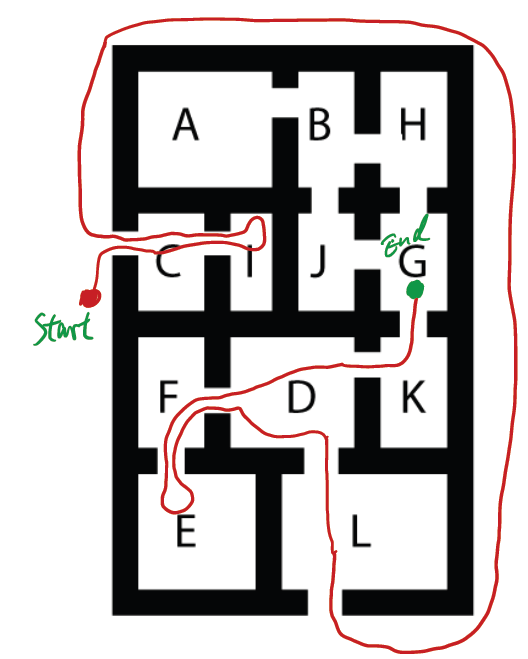
\includegraphics[width=0.3\columnwidth]{DFStraceG}\centering 
\caption{Illustrating tracing a DFS on G starting at U route}
\end{figure}
\item The drone takes 4 minutes to scan a room and 2 minutes to move from one room to another.  The drone needs 7 minutes to move from \textsf{L} to \textsf{C} (or {\it vice versa}).  What is the approximate total time it takes for the drone to check the floor?  How would you annotate the graph to reflect this cost? ({\it You're not asked to redo the graph--just explain what you'd do})\\
\underline{Answer to question 3(d):}\\
I would like to define Edge weight as path cost representing the time from one room to another. And on each node(vertice), I would mark the cost which is represent the time to scan the room(for U, it is pass U). So it would be like as the following figure: since for some room it needs back and forth, for example,room C and room I. And the robot need to back to U after checking, So total time is 12*4+1*7+22*2=99 minutes\\
\begin{figure}[h]
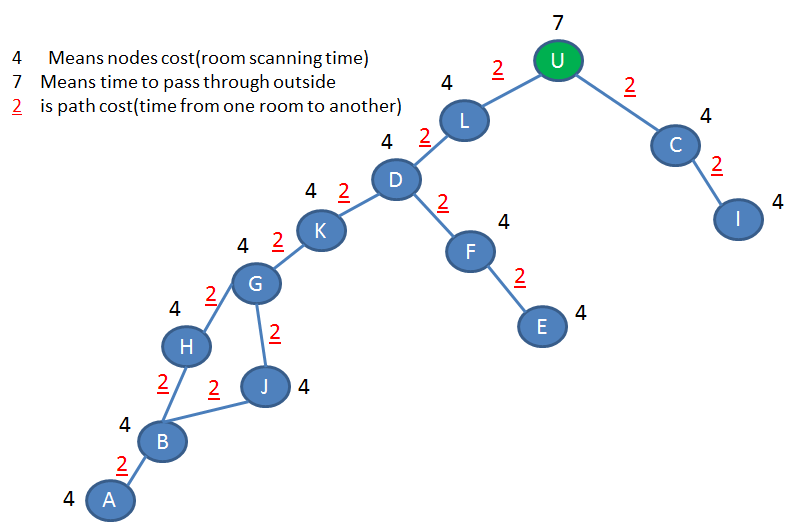
\includegraphics[width=0.5\columnwidth]{graphp3withcost}\centering 
\caption{Illustrate the floor plan with graph with cost}
\end{figure}
\item A single battery for the drone holds about 45 minutes worth of charge.  How many batteries does the drone need to scan the floor?\\
\underline{Answer to question 3(e):}\\
Since it takes 99 minutes, so it needs 3 batteries.\\
\item Using Python, create an adjacency list data structure (I used a dictionary which seems reasonable); then using either a Python package or your own implementation, do a DFS from the {\it outside} of the floor, {\it i.e.,} DFS($G$, \textsf{U}).  The DFS should yield a sequence of rooms that the drone would scan.\\
\underline{Answer to question 3(f,g,h): here it is running result with python script}\\
\begin{figure}[h]
{\small
\begin{verbatim}
0 scan room: U scan&movetime:  0 Accumulatetime: 0
1 scan room: L scan&movetime:  6 Accumulatetime: 6
2 scan room: D scan&movetime:  6 Accumulatetime: 12
3 scan room: F scan&movetime:  6 Accumulatetime: 18
4 scan room: E scan&movetime:  6 Accumulatetime: 24
Returnpath:  ['E', 'F', 'D', 'K'] movetime: 4 Accumulatetime: 28
5 scan room: K scan&movetime:  6 Accumulatetime: 34
Warning! Please change your battery:  5 mins left
Congratulations! 2 th New Battery is loaded successfully
6 scan room: G scan&movetime:  6 Accumulatetime: 40
7 scan room: H scan&movetime:  6 Accumulatetime: 46
8 scan room: B scan&movetime:  6 Accumulatetime: 52
9 scan room: J scan&movetime:  6 Accumulatetime: 58
Returnpath:  ['J', 'B', 'A'] movetime: 2 Accumulatetime: 60
10 scan room: A scan&movetime:  6 Accumulatetime: 66
Warning! Please change your battery:  0
Congratulations! 3 th New Battery is loaded successfully
Returnpath:  ['A', 'B', 'H', 'G', 'K', 'D', 'L', 'U', 'C'] movetime: 19 Accumulatetime: 85
11 scan room: C scan&movetime:  6 Accumulatetime: 91
12 scan room: I scan&movetime:  6 Accumulatetime: 97
Returnpath:  ['I', 'C', 'U'] movetime: 2 Accumulatetime: 99
Totaltime:  103
Batteryused: 3
27 mins battery left
\end{verbatim}}
\end{figure}
\item Add the cost to the drone and battery life to the search; when the drone has scanned all the rooms, give the percent battery life left. 
\item  Presume the drone starts and ends at \textsf{U}.
\end{enumerate}
\item Rock/Paper/Scissors is a simple game: numbers 0,1,2 denotes each of these items with an outcome that rock {\it beats} scissors, scissors {\it cut} paper, and paper {\it covers} rock; otherwise it's a tie.  Included below (and as file) is a Python script that allows a human to play with a computer. 
\begin{figure}[h]
{\small
\begin{verbatim}
import random as rn
#values of rock, paper, scissors
r,p,s = 0,1,2
#dictionary e.g., rock beats scissors
ws = {r:s, p:r, s:p}
nogames = int(input("Number of games? "))
totgames = 0
compwins = 0
humwins = 0
ties = 0
gamehistory = []
while totgames < nogames:
     human = int(input("r=0,p=1,s=2 "))
     comp = rn.randrange(0,3,1)
     gamehistory.append([human, comp])
     print("Human: {0}, Comp: {1}".format(human, comp))
     if ws[comp] == human:
        compwins += 1
     elif ws[human] == comp:
        humwins += 1
     else:
        ties += 1
     totgames += 1
v = list(map(lambda x: 100*x/totgames, [compwins, humwins, ties]))
print("Stats\ncw% = {0}, hm% = {1}, ties% = {2}".format(*v))
\end{verbatim}}
\end{figure}
\begin{enumerate}
\item Play 5 times of 10 games (it will go quickly) and record the statistics for your wins, $H_1, H_2, \ldots, H_5$.   {\it Expectation} gives us a measure of central tendency (sometimes called the mean).  We can calculate the expectation as
\begin{eqnarray*}
\mathrm{E}[H] &=& \sum_{i=1}^5 H_i/5
\end{eqnarray*}
What is the expecation of a human winning? Are you surpised? Of the computer winning?\\
\underline{Answer to question 4(a):}\\
Here it is the record about running 5 times of 10 games:
\begin{verbatim}
computer wins: [5, 5, 3, 1, 4] human wins: [2, 3, 4, 4, 1] ties: [3, 2, 3, 5, 5]
ncw E= 3.6, hm E = 2.8, ties E = 3.6
\end{verbatim}
The expectation for human to win the game is a little bit low: $28\%$.\\
The expectation for computer to win the game is higher than human which is $36\%$.\\
Here it is part of code to call the function(5 times) provided by instructor:$rps\_game$. For full code, please refer to attachment file $py2\_1\_jinjujiang.py$
\begin{verbatim}
n=5
sumwinh=0
sumwinc=0
sumwint=0
for i in range(n):
    h,c,t=rps_game(10)
    H.append(h)
    sumwinh +=h
    C.append(c)
    sumwinc +=c
    T.append(t)
    sumwint +=t
print("computer wins:",C,"human wins:",H,"ties:",T)
v = list(map(lambda x: x/n, [sumwinc, sumwinh, sumwint]))
print("ncw E= {0}, hm E = {1}, ties E = {2}".format(*v))
\end{verbatim}
\item From \url{python.org} look-up the random function.  How is it picking the numbers 0,1,2?  Does the computer's choice of numbers depend on its previous choice? How about a yours?\\
\underline{Answer to question 4(b):}\\
This module implements pseudo-random number generators for various distributions.For integers, uniform selection from a range.\\
Here I just checked the computer's choices and plot it:  Although it looks like that computer's choice does not depend on previous choices. However,In theory, any pseudo random number generator can be figured out from the outside looking in, although in practice, a strong pseudo random number generator will take a very impractical amount of time.So it is possible to predict the next number based on previous numbers.And it also means that the computer's choice of number can be predicted from its previous choices.That is why there is warning in python.org:The pseudo-random generators of this module should not be used for security purposes. Use os.urandom() or SystemRandom if you require a cryptographically secure pseudo-random number generator.\\
And as to human's choice, it does depends on previous choices. For example, If my choice is rock, then there is lower possibility to show rock next time. \\

\item Remove the human player and add another computer player called Robby.  See if you can find a strategy that has Robby's expected winning greater than the computer.  You are free to employ whatever you'd like so long as it's yours.\\
\underline{Answer to question 4(c):}\\
\textbf{Strategy 1:} Record computer's previous choices, and get the most common choices, assuming that computer's next choice will not be the same. For example, if the most common choice is rock, then I would assume that computer's next choice will not be rock, so Robby's choice can be scissors.
By using this strategy, Robby's the winning expectation is higher than human player, but it not always getting higher winning expectation than computer.\\
\underline{here it is some running results for strategy 1($p2\_2\_jinjujiang.py$):}\\
50 times(10 games):\\
ncw E= 2.96, Robby E = 3.5, ties E = 3.54\\
\textbf{Strategy 2:} Assuming computer's choice will be similar as human: next choice will be different than previous choice. By using this strategy, sometimes Robby can win computer, sometimes not. here it is part of python script:
\begin{verbatim}
    if(len(gamehistory)==0):
        Robby = rn.randrange(0,3,1)
    else:
        Robby = ws[gamehistory[-1][0]]
\end{verbatim}
\textbf{Strategy 3:} Setup seed, then Robby will definitely win!$p2\_3\_jinjujiang.py$(but it is also like cheating.)
\begin{verbatim}
ncw E= 3.0, Robby E = 7.0, ties E = 0.0
\end{verbatim}
\end{enumerate}
\end{enumerate}
\end{document}
